\section{Predicato}
Esprime una proprietà che un oggetto di un gruppo può avere o non avere o relazioni tra gli oggetti di un gruppo.
\begin{example}
$P(x, y)$ \textit{x} ama \textit{y} \\
\emph{Luca ama Laura}
\end{example}

Il predicato \textit{P} è una funzione con dominio l'universo del discorso e codominio il valore \textbf{T} o \textbf{F}.

\section{Quantificatori}
Essi vengono usati per esprime una proprietà su un gruppo di oggetti o l'esistenza di un oggetto con una proprietà in un gruppo.

\subsection{Universale}
Il quantificatore $\forall$ viene usato per esprimere una proprietà su un gruppo di oggetti. Per essere \textbf{T}, tutti gli oggetti nel dominio devono rispettare le proprietà.
\begin{example}
\emph{Tutti i laureati in informatica hanno fatto l'esame di MMI} \\
$P(x)$, \textit{x} è laureato in informatica \\
$Q(x)$, \textit{x} ha fatto l'esame di MMI \\
Dominio di \textit{x} sono tutti gli umani \\
$\forall xP(x) \implies Q(x)$
\end{example}

\textbf{N.B:} Se $\forall xP(x)$ è falso, ciò \underline{non} significata che tutti gli oggetti del dominio di \textit{x} non rispettino la proprietà \textit{P}, ma che esiste almeno un oggetto che non rispetta le proprietà.

\subsection{Esistenziale}
Il quantificatore $\exists$ viene usato per esprime l'esistenza di un oggetto con una determinata proprietà in un gruppo di oggetti. Affinché sia \textbf{T}, deve esistere almeno un oggetto che rispetti le proprietà.
\begin{example}
\emph{Alcuni laureati in informatica hanno fatto l'esame di programmazione avanzata} \\
$P(x)$, \textit{x} è laureato in informatica \\
$Q(x)$, \textit{x} ha fatto l'esame di programmazione avanzata \\
Dominio di \textit{x} sono tutti gli umani \\
$\exists xP(x) \wedge Q(x)$
\end{example}

\subsection{Dominio vuoto}
Se il dominio del predicato $P(x)$ è $\emptyset$, i quantificatori hanno i seguenti comportamenti: 
\begin{itemize}
    \item $\forall xP(x)$: è \textbf{T} in quanto non si può trovare un controesempio per dimostrare che è \textbf{F}.
    \item $\exists xP(x)$ è \textbf{F} in quanto non si può trovare un esempio per dimostrare che è \textbf{T}.
\end{itemize}

\subsection{Cambio dominio}
Se si cambia il dominio di un predicato, il valore di verità dell'intera proposizione può cambiare totalmente.
\begin{example}
\emph{Alcuni laureati in informatica hanno fatto l'esame di programmazione avanzata} \\
$P(x)$, \textit{x} ha fatto l'esame di programmazione avanzata \\
Dominio di \textit{x} tutti i laureati in informatica.
Allora avremmo che $\exists xP(x)$ è \textbf{T}. \\
Se cambiamo il dominio di \textit{x} in tutti i laureati di filosofia, avremmo che  $\exists xP(x)$ è \textbf{F}.
\end{example}

\subsection{Quantificatori innestati}
I quantificatori $\forall$ e $\exists$ si possono combinare tra di loro per formare predicati più complessi.
\begin{example}
\emph{Ogni figlio ha una madre} \\
$P(x)$, \textit{x} è un figlio \\
$Q(x)$, \textit{x} è una madre \\
$R(x, y)$, \textit{x} è figlio di \textit{y} \\
Dominio di \textit{x} e \textit{y} sono tutti gli umani \\
$\forall x \exists y \mid R(x, y) \wedge P(x) \wedge Q(y)$
\end{example}
\begin{example}
\emph{Ognuno apprezza qualcuno} \\
$P(x, y)$, \textit{x} apprezza y \\
Dominio di \textit{x} e \textit{y} sono tutti gli umani \\
$\forall x \exists y \mid P(x, y)$
\end{example}

\subsection{Negazione quantificatori}
I quantificatori possono essere negati. La regola generale è che se il quantificatore è $\forall$, diventa $\exists$ e viceversa e poi si nega il predicato.
\begin{itemize}
    \item $\neg(\forall xP(x)) \equiv \exists x \neg P(x)$
    \item $\neg (\exists xP(x)) \equiv \forall x \neg P(x)$
\end{itemize}

\subsubsection{Negazione quantificatori innestati}
La regola generale è che si cambiano i quantificatori con il loro opposto e si nega il predicato.
\begin{example}
$\neg(\forall x(P(x) \implies Q(x))) \equiv$ \\
$\exists x \neg(P(x) \implies Q(x)) \equiv$ \\ 
$\exists x \neg(\neg P(x) \vee Q(x)) \equiv$ \\
$\exists x(P(x) \wedge \neg Q(x))$
\end{example}
\begin{example}
Negare il seguente predicato $\forall x(x > 0 \implies \exists y \mid (x \cdot y=1))$ \\
$\neg(\forall x(x > 0 \implies \exists y \mid (x \cdot y=1))) \equiv$ \\
Si può spostare $\exists y$ all'inizio, in quanto lo scope di y non cambierebbe e risulta più facile la negazione \\
$\neg(\forall x(x > 0 \implies \exists y \mid (x \cdot y=1))) \equiv$ \\
$\neg(\forall x \exists y(x > 0 \implies (x \cdot y=1))) \equiv$ \\
$\exists x \forall y \neg(x > 0 \implies (x \cdot y=1))) \equiv$ \\
$\exists x \forall y \neg(\neg (x > 0) \vee (x \cdot y=1)) \equiv$ \\
$\exists x \forall y((x > 0) \wedge \neg (x \cdot y=1)) \equiv$ \\
$\exists x \forall y((x > 0) \wedge (x \cdot y \neq 1))$
\end{example}

\subsection{Dominio finito}
Se il dominio del predicato è finito ed è presente un quantificatore, esso può essere anche rimosso a seconda del quantificatore e la proposizione continuerà ad avere lo stesso valore di verità.
\begin{example} Supponiamo che il dominio del predicato $P(x)$ abbia \textit{n} oggetti. Avremmo che le seguenti equivalenze sono \textbf{T}:
\begin{itemize}
    \item $\forall xP(x) \iff P(x_1) \wedge P(x_2) \wedge ... \wedge P(x_n)$
    \item $\exists xP(x) \iff P(x_1) \vee P(x_2) \vee ... \vee P(x_n)$
    \item Funzione proposizionale $Q(x, y)$ con dominio $\{1, 2\} \times \{1, 2\}$ \\
    $\exists x \forall y Q(x, y) \iff (Q(1,1) \wedge Q(1, 2)) \vee (Q(2,1) \wedge Q(2, 2))$
    \item Funzione proposizionale $Q(x, y)$ con dominio $\{1, 2\} \times \{1, 2\}$ \\
    $\forall x \exists y Q(x, y) \iff (Q(1, 1) \vee Q(1, 2)) \wedge (Q(2, 1) \vee Q(2, 2))$
\end{itemize}
\end{example}

\section{Insieme di verità}
L'insieme di verità di $P(x)$ è l'insieme degli elementi $x_i$ nel dominio di $P(x)$ tali che $P(x)$ è \textbf{T}.

In termini matematici l'insieme di verità rappresenta un sottoinsieme della controimmagine di $P(x)$ tale che $P(x)=$ \textbf{T} \\
Il codominio di $P(x)$ è $C=\{T, F\}$, sia $D$ il dominio di $P(x)$, $V$ l'insieme di verità di $P(x)$ e $A=\{T\}\subset C$. \\
Si ha che l'insieme di verità di $P(x)$ è $f^{-1}(A)=\{x\in D \mid P(x)=T\}=V$
\begin{figure}[H]
\centering
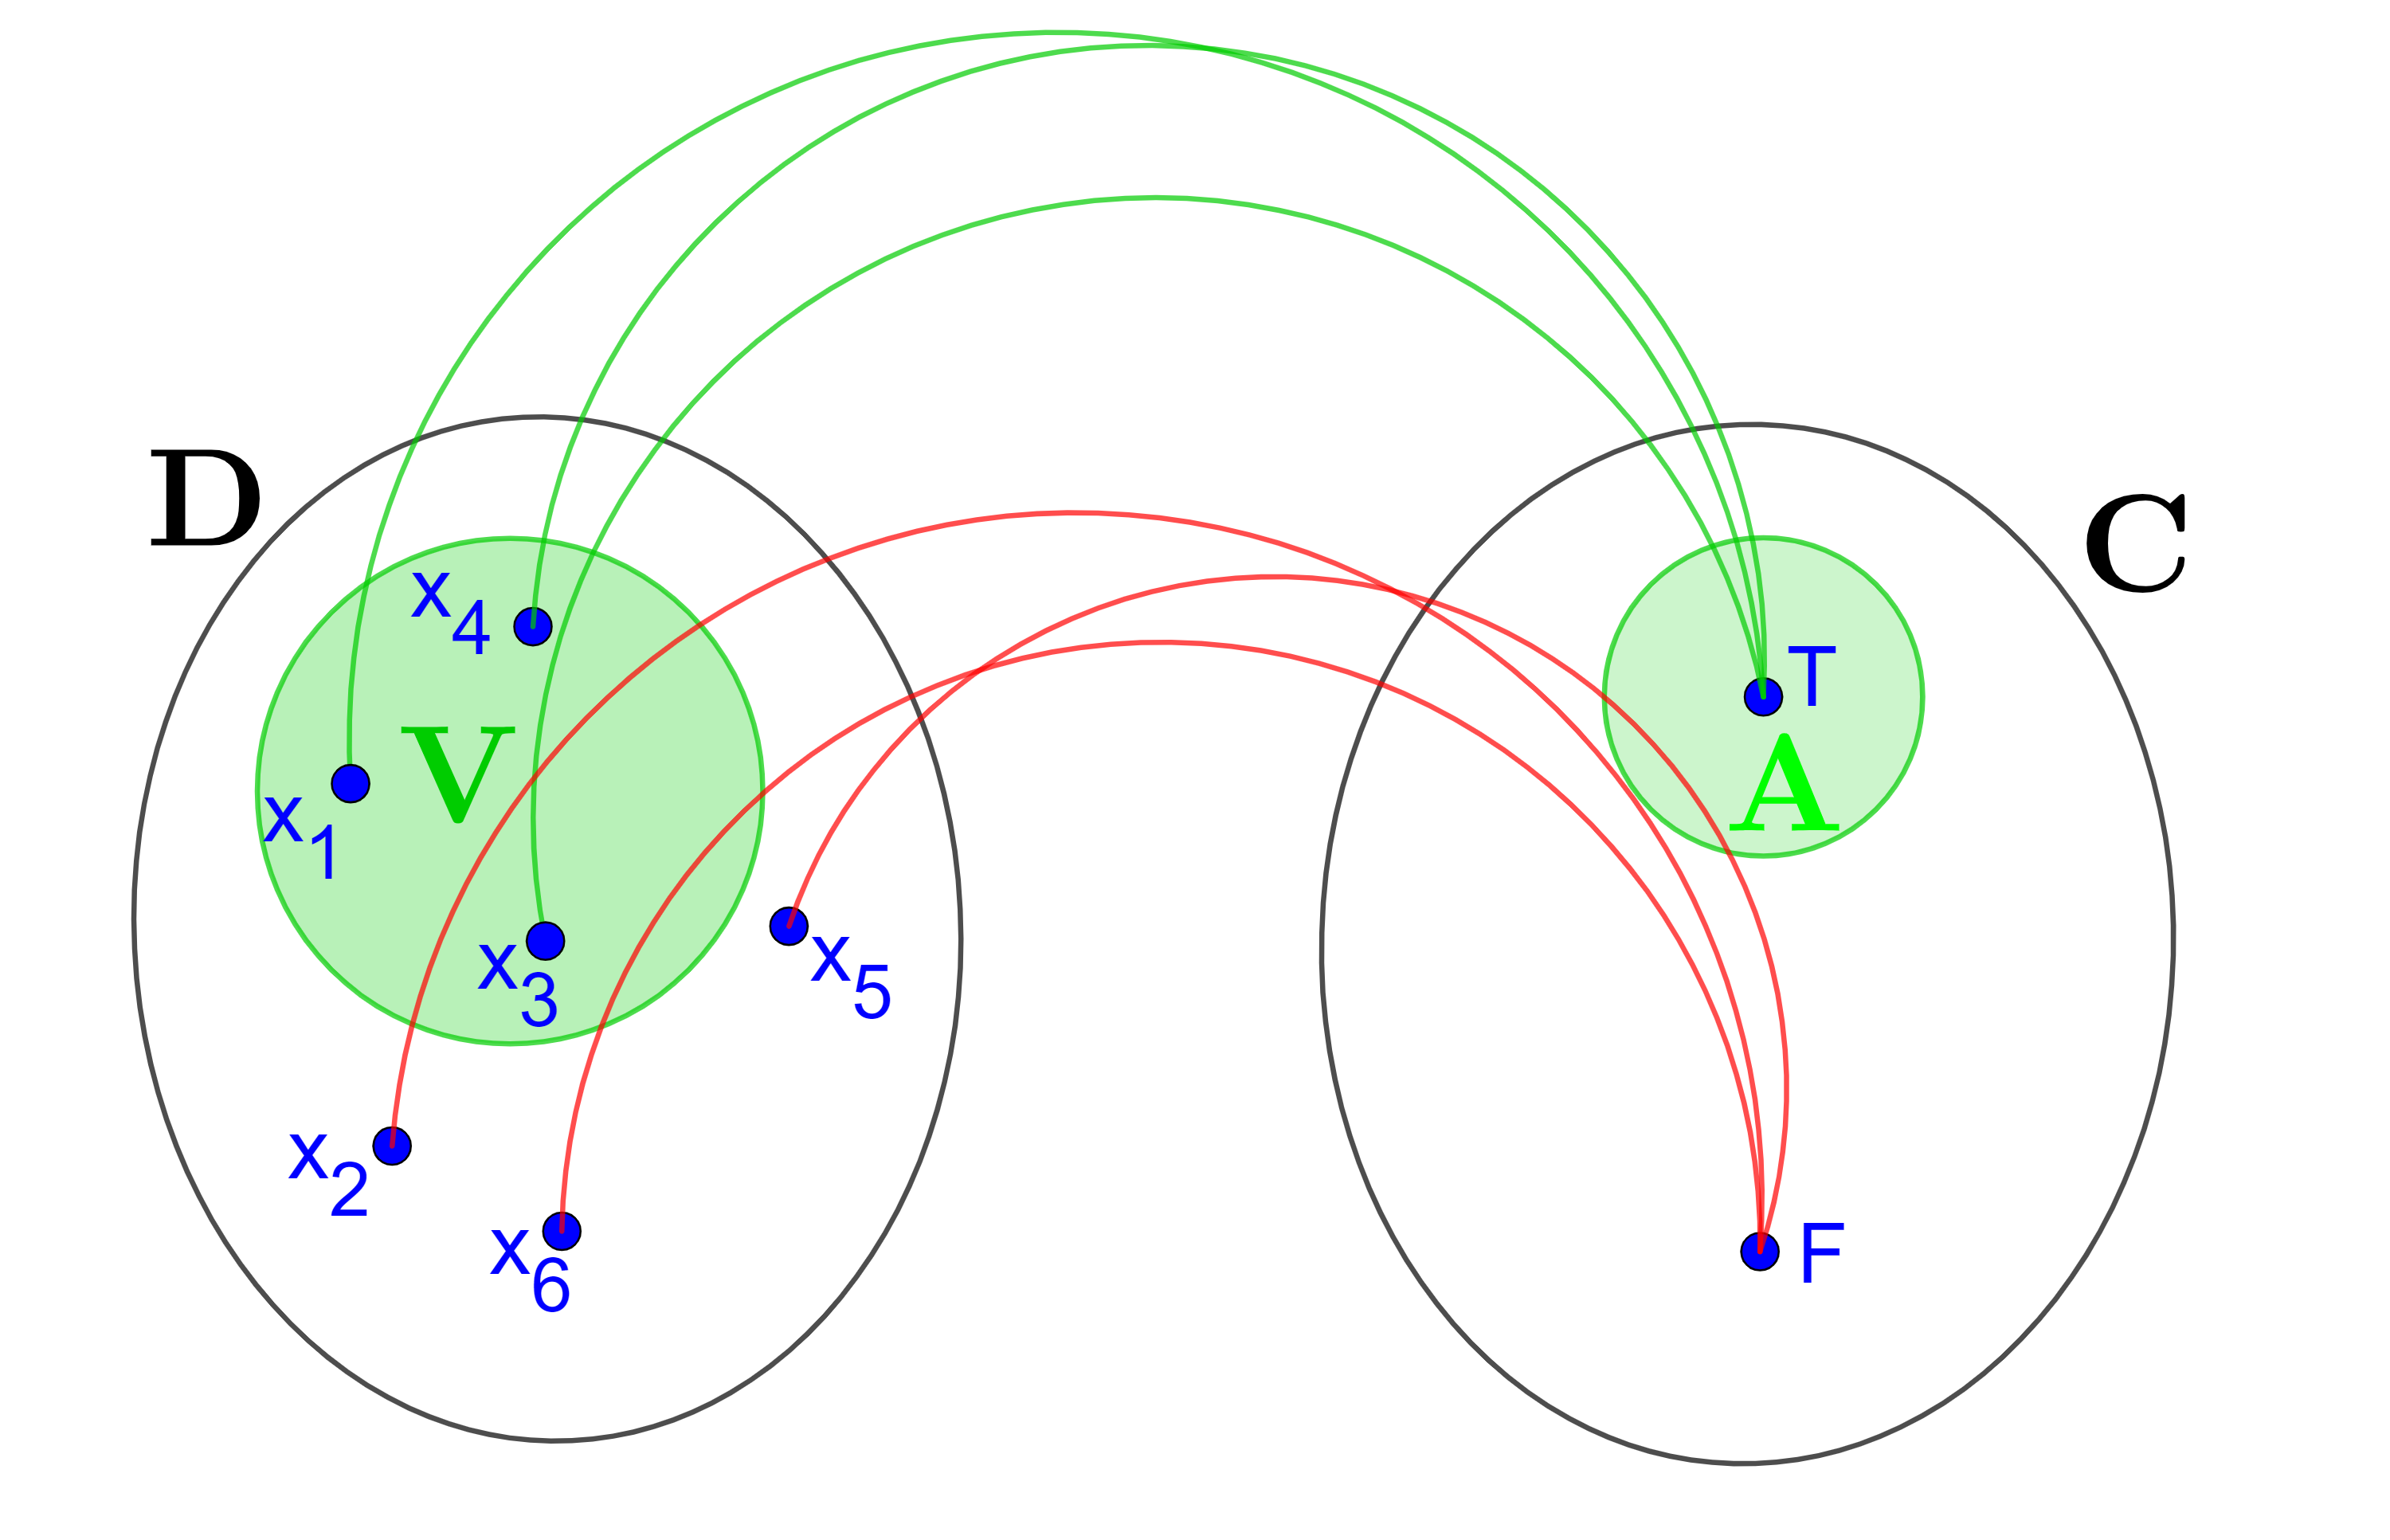
\includegraphics[scale=1.7]{chapters/logica_predicativa/figure_insieme_verita}
\caption{Rappresentazione grafica esempio di insieme di verità.}
\end{figure}